\chapter{Reinforcement Learning Approaches}
\label{chap:reinforcementlearning}
This chapter describes two \ac{RL} approaches used to tackle the important problem of optimized trade execution. Based upon the \ac{RL} formulation, as described by Nevmyvaka \etal \cite{Nevmyvaka:2006}, Q-learning and dynamic programming are fused to find an optimal, state-based strategy from a training set of historic orderbook data. While sampling the discretized state space\footnote{The state space describes actual trade progress (\ie \emph{remaining time} and \emph{remaining inventory}) as well as current market situation.} in a backward, brute force manner, the authors achieved an impressive 50\% gain over the more simple Submit \& Leave Strategy (see \Cref{chap:tradingstrategies}). The novel, forward-learning approach proposed in this work, outperforms the original method, as it samples from the continuous state space through forward exploration in order to generate more realistic transitions.\\

Some of the assumptions made in the original, backward approach deserve a closer look and motivate for modifications. As the authors assessed a rather large, proprietary dataset of 1.5 years of millisecond time-scale limit order data from \acs{NASDAQ}, it is furthermore intriguing to evaluate its performance on a smaller, self-recorded dataset of limited resolution.






\section{General Framework}
\label{chap:reinforcementlearning:original}
In the first place, the general framework of the reinforcement learning problem is described.


\subsection{State space}
\label{chap:statespace}
The state space consists of various variables, describing the current trade progress (\emph{private variables}) and the current market situation as observable from orderbook data (\emph{market variables}). The two private variables \emph{remaining time} (\lstinline!time!) and \emph{remaining inventory} (\lstinline!volume!) make the base for all subsequent experiments, while optional market variables may be enclosed to potentially assist the process of decision finding.\\

Each \lstinline!state! $s \in <volume, time, o_1, o_2, ...>$ forms a vector of at least both private variables, plus a variable number of market variables. More specifically, the following market variables may be added to the state space to further improvement the cost reducing capabilities of the strategies obtained over plain \lstinline!VolTime!-strategies.

\begin{description}
\item[Bid-Ask Spread]: Spread between best bid price and best ask price.
\item[Bid-Ask Volume Misbalance]: Volume imbalance between orders at the best bid price and the best ask price.
\item[Immediate Market Order Cost]: Costs, if remaining volume would be executed immediately, at the current market price.
\item[Signed Transaction Volume]: Signed volume of all trades executed within the last 15 seconds. A positive value indicates more buy orders, while a negative value complies to more sell orders being executed.
\end{description}

Except for \emph{Immediate Market Order Cost}, the market variables originally exploited basically stem from market level 1 data only. In addition to the above mentioned market variables, the impact of additional market level 2 features, describing potential imbalances between ask and bid book and forecasting estimated action consequences is examined.
\begin{description}
\item[marketPrice] : Relative difference between current center price and the worst price that must be paid (or is received) in case of simple market orders.

\item[sharecount] : Number of Bitcoins, immediately available for the specified amount of cash.

\item[center\_price] : Current center price.

\item[\_a*\_effects] : Minimum cash volume immediately tradeable by individual actions. The value is a lower bound estimate of the true volume, because only the current orderbook is retrievable. New opportunities, arising within the forthcoming \lstinline!trading_period! are unacquainted and thus not included.
\end{description}

In the original approach, market variables are discretized into 0 (low), 1 (medium) and 2 (high), while the concrete category mapping process is not further described. In this work, market variables are evenly transformed into $N$ bins $o_m \rightarrow o_m\_discN$, where boundaries between bins are automatically derived from the respective training data quantiles. Private variables are discretized in 4 to 8 bins, while greater resolutions lead to strictly better results and linearly higher computation times.


\subsection{Action space}
\label{chap:actionspace}
Actions define the level of trading aggression to be performed. In the original approach, action $a \in \mathbb{R}$ defines the deviation between current best price and chosen limit price, as $bid + a$ (for buy orders) and $ask - a$ (for sell orders). As such, actions must cross the full bid-ask-spread to find matching orders in the opposing book. Large actions $a$ result in larger fractions of the order volume being matched immediately. Smaller or even negative actions $a$ help to prolong the actual execution, and may help to profit from opportune market movements.\\

In case of the exemplary market situation shown in \Cref{table:orderbook:example:again}, a buy order with an aggressive action $a=1.4$ would map into $limit=bid+a=28.7+1.4=30.1$. This limit would allow trading up to 75 shares instantaneously.\\

\begin{table}
\centering
	\scalebox{0.8}{
\rowcolors{1}{}{black!5}
\begin{tabular}{|RRcRRR|}
\toprule
{} &  \text{Amount} &    Type &  \text{Volume} &  \text{VolumeAcc} &  \text{norm\_Price} \\
\midrule
31.00 &   200.0 &     ask &  6200.0 &     8425.0 &    1.074533 \\
30.00 &    50.0 &     ask &  1500.0 &     2225.0 &    1.039871 \\
29.00 &    25.0 &     ask &   725.0 &      725.0 &    1.005208 \\
28.85 &     NaN &  center &     NaN &        NaN &         NaN \\
28.70 &   200.0 &     bid &  5740.0 &     5740.0 &    0.994810 \\
28.50 &   100.0 &     bid &  2850.0 &     8590.0 &    0.987877 \\
28.00 &   300.0 &     bid &  8400.0 &    16990.0 &    0.970546 \\
\bottomrule
\end{tabular}
}
\caption{Action $a=1.4$ translates into $limit=28.7 + 1.4 = 30.1$.}
\label{table:orderbook:example:again}
\end{table}

The employed number of selectable actions and their actual value range was not further specified.\\

As the proposed mapping method do not necessarily fit well to the bitcoin data at hand, two modifications are made: On the one hand, Bitcoin prices have burst from roughly 700\$ to more than 2.000\$ in the period of recording (see \Cref{fig:ploniexPriceHistory}), \ie interpreting actions as the absolute difference to the current best prices, maps to significantly different levels of aggression as time passes. On the other hand, the large volatility of Bitcoins (see \Cref{fig:bitcoinvolatility}) causes rapid fluctuations in the bid-ask spread as a side effect. Fixing the limit base to the opposing best price, the spread must no longer be crossed and action $a=0$ now generally refers to the first action that causes a guaranteed execution volume larger than zero.\\


The mapping functions are thus redefined as follows:\\
\lstinline!limit_buy = ask * (1 + (a/1000))! instead of \lstinline!limit_buy = bid + a!\\
\lstinline!limit_sell = bid * (1 - (a/1000))! instead of \lstinline!limit_sell = ask - a!\\

Typically the following set of fifteen actions is used: $L=[-4,-3,..,9,10]$, where \eg action $a=4$ translates into $limit = ask * 1.004 = ask + 0.4\%$. 


\subsection{Costs}
\label{chap:costs}
Costs are defined as the slippage induced from the previously chosen actions. The baseline is given by the initial center price. The following formula is used to compute (partial) costs in terms of price deviation from the idealized case of buying all shares at the initial center price:
\begin{equation}
\label{eq:imcost}
   cost_{im} = (avg\_paid - initial\_center) * volume\_traded
\end{equation}
\begin{equation}
   initial\_center = (\dfrac{ask_t+bid_t)}{2} | t=0
\end{equation}

Since the complete trade execution happens within a finite time horizon and full execution of the \lstinline!volume! is mandatory, partial costs can simply be summed up without any discounting. Utilizing the \ac{OTS}, it is not possible to compute occurring costs in advance exactly, as they depend on how the market evolves within the subsequent \lstinline!trading_period!.\\

\begin{wrapfigure}{r}{0.35\textwidth}
	\centering
	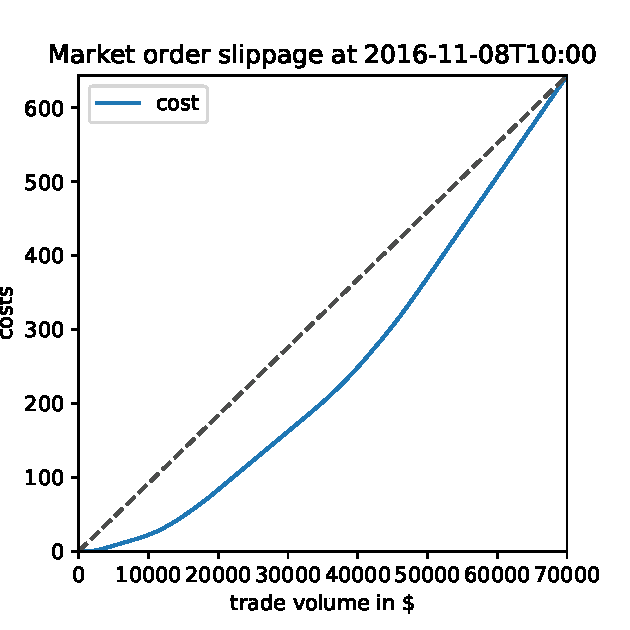
\includegraphics[width=0.3\textwidth,trim={0 0.2cm 0 0.7cm},clip]{content/drawings/nonlinearcosts}
	\caption{Non-linear slippage growth.}
	\label{fig:nonlinearcosts}
\end{wrapfigure}

While discretization of market variables mainly affects the strategies explanatory power, the resolution of private variable \lstinline!volume! leads to considerable rounding issues in regards to the cost function employed. As observed successor states $x_{t-1}$ must be discretized equally to allow looking up the corresponding minimal costs, the immediate costs, as computed in \Cref{eq:imcost}, must be scaled accordingly. Simply replacing \lstinline!volume_traded! with \lstinline!round(volume_traded)! falsifies the actual costs, as they correlate to the accomplished trade volume in an  unpredictable, non-linear manner as indicated in \Cref{fig:nonlinearcosts}.\\

Nevmyvaka \etal \Cite{Nevmyvaka:2006} did not mention this problematic and presumably did not perform any cost scaling at all. Despite the non-linear relationship between trading volume and observed costs, this simple, but imprecise approach of \emph{linear cost scaling} is used in all discrete state spaces examined.

\subsection{Subject of Trade}
\label{chap:backwardalgorithm:discussion:subjectTrade}
Nevmyvaka \etal \cite{Nevmyvaka:2006} tackled the problem of trading a certain amount of shares within a fixed time period. A more practicable problem definition must distinguish between the concrete trading direction. While their problem definition fits to the case of selling shares that are in the investors possessions, it does not mirror the opposite case properly. If the subject of trade is to obtain shares, it is more realistic to define a fixed amount of disposable \emph{cash}, rather than the number of \emph{shares}, that shall be acquired. Subsequently, all experiments in buy direction are instructed to commute a fixed amount of cash into as many shares as possible.\\
 
If cash is the subject of trade, the optional market variable \emph{Immediate Market Order Cost}  (\eg $72.321\$$) becomes meaningless, and is replaced by \emph{Immediate Market Order Shares} (\eg 92 BTC), displaying the number of shares acquirable through an immediate market order.



\section{Backward Learning}
\label{chap:backwardlearning}
In order to learn the optimal limit for each possible situation, orderbook windows are examined in a backward, brute-force manner as described in \Cref{alg:bruteforce:pseudocode}. Each orderbook window from the training data set is sampled $T*I*L$ times, where $T$ is the number of performed limit revisions, $I$ is the number of discrete volume states and $L$ is the number of available actions.\\

\begin{algorithm}[H] 
 \caption{Optimal\_strategy\Cite{Nevmyvaka:2006}.}
     \SetAlgoLined
     \footnotesize
     
     \KwIn{V=70.000\$, H=60min, T=4, I=[12.5\%..100\%], L=[-4..10]}

\For{t=1 to T}{
    \While{not end of data}{
        Transform (orderbook) $\rightarrow o_1..o_R$\;
        \For{i=0 to I}{
            \For{a=0 to L}{
                 Set $x = [t, i, o_1, ..., o_R]$\;
                    Simulate transition $x \rightarrow y$\;
                    Calculate immediate $\text{cost}_{im}(x, a)$\;
                    Look up argmax $\text{cost}(y, p)$\;
                    Update $\text{cost}([t, v, o_1, ..., o_R], a)$\;

            }
        }
        Select the highest-payout action argmax $\text{cost}(y, p)$ in every state $y$ to output optimal policy
    }
}
\label{alg:bruteforce:pseudocode}
\end{algorithm}\bigskip

While the algorithms running time depends solely on the resolution of the two private variables, the chosen action space and the size of the training data set, it is approximately independent of the number of market variables chosen. For the transition simulation, the model described in \Cref{chap:tradeexecution} is utilized. The cost update rule is given below: 
\begin{equation}\label{eq:costfunction}
   cost(x_t, a) = \dfrac{n}{n+1} cost(x_t, a) + \dfrac{1}{n+1} [cost_{im}(x_t,a) + \arg\min_{p}cost(x_{t-1}, p)]
\end{equation}

The algorithm assumes the individual trading periods to be of an (approximately) Markovian nature, where the optimal action to choose at state $x_t$ with $t = \tau$ is completely independent of actions chosen previously ($t \geq \tau$).\\

As such, the state-action function can be computed inductively via dynamic programming. In a first round, expected costs for all actions in states being immediate predecessors of end states (\ie $t=1$) are computed according to \Cref{eq:costfunction}. \Cref{fig:heatmap:t1} visualizes the resulting optimal costs (right) and corresponding actions (left) after the first round has finished.

\begin{figure}[ht]
	\centering
   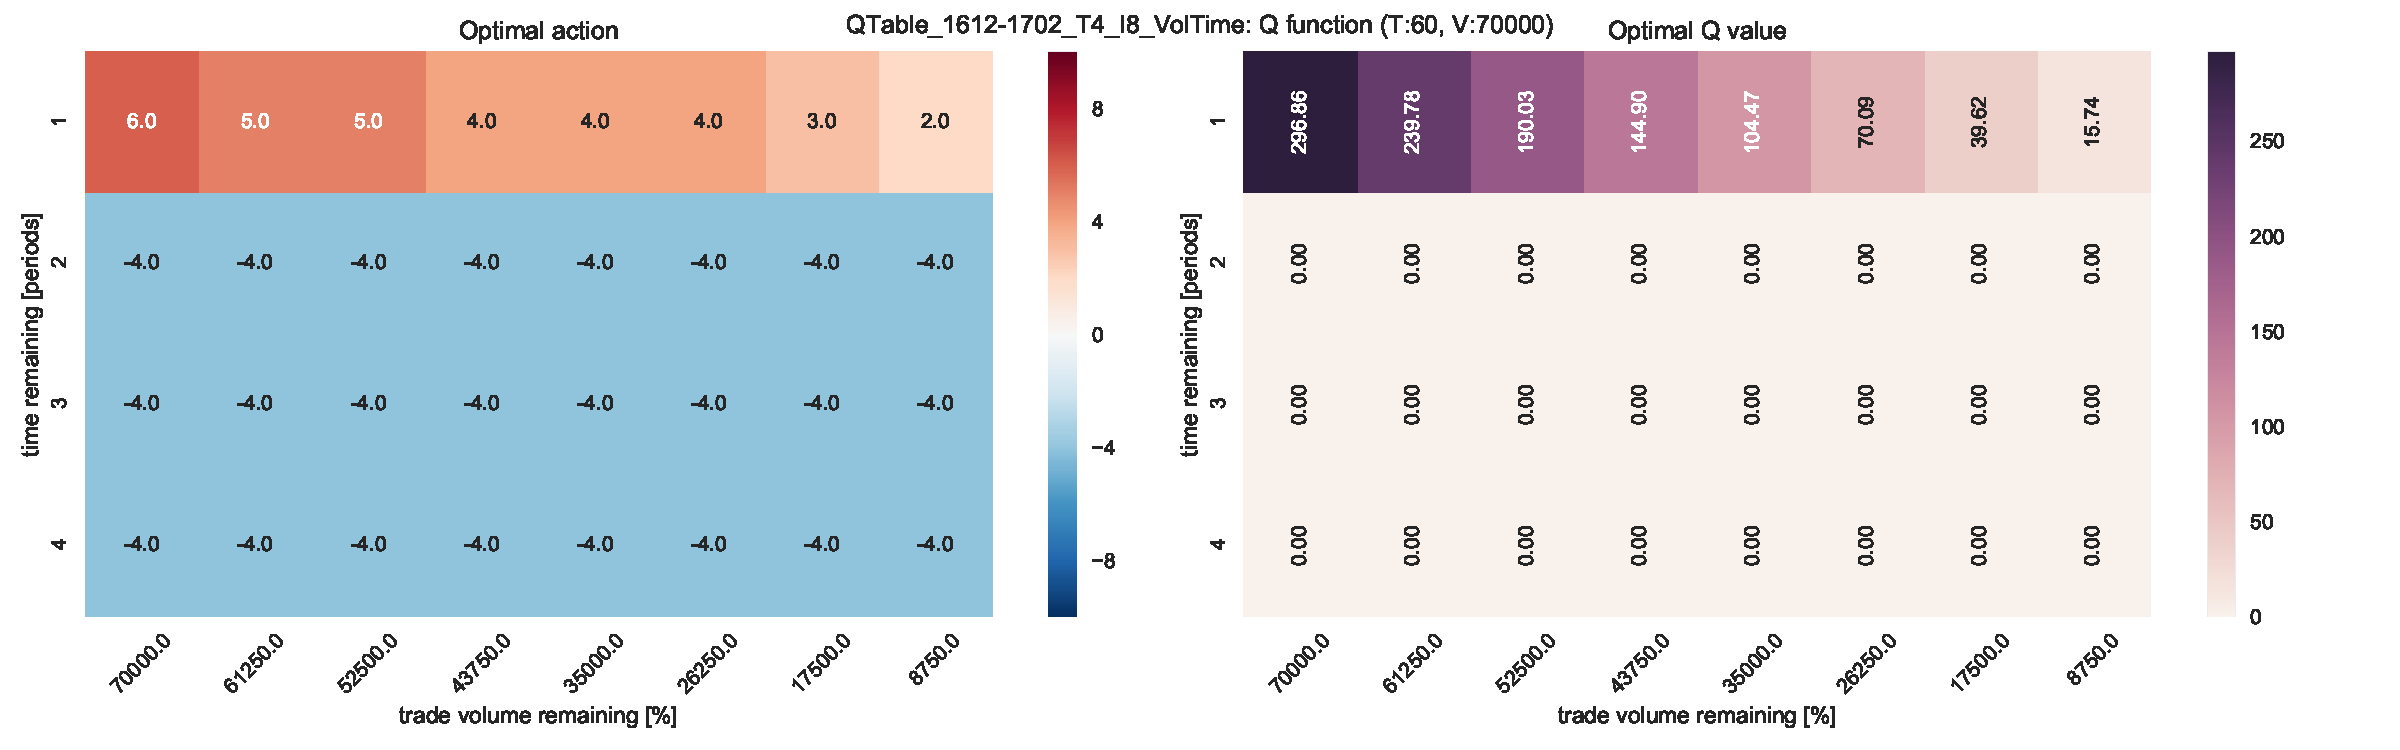
\includegraphics[width=0.8\textwidth]{content/drawings/heatmap_3months_t1}
	\caption{State-Action function, visualized after the first training round.}
	\label{fig:heatmap:t1}
\end{figure}

Knowing the optimal state-action values for all states with $t=1$, all informations are given to compute the optimal state-action values for their predecessor states with $t=2$ (see \Cref{fig:heatmap:t2}).

\begin{figure}[ht]
	\centering
   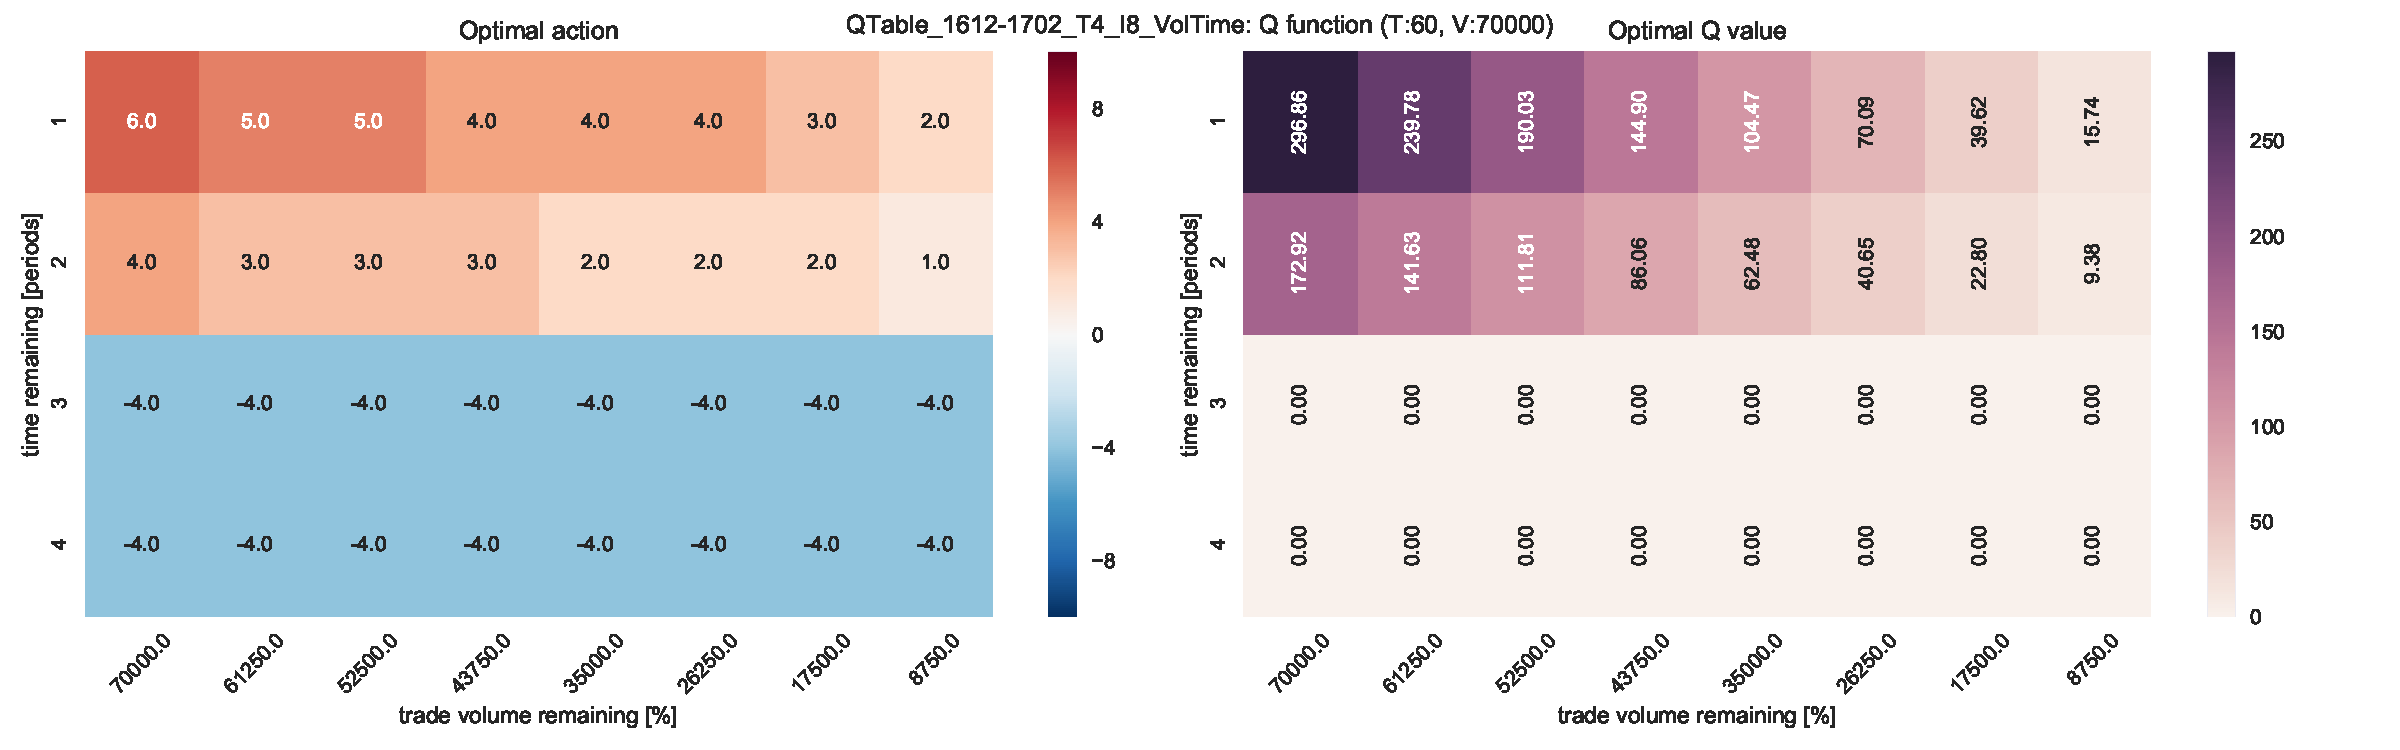
\includegraphics[width=0.8\textwidth]{content/drawings/heatmap_3months_t2}
	\caption{State-Action function, visualized after the second training round.}
	\label{fig:heatmap:t2}
\end{figure}

After $T$ iterations a globally optimal policy, as shown in \Cref{fig:heatmap}, has been found. The annotated q values (right) denote the corresponding minimum over all available actions. The visualized state-action function was trained over orderbook snapshots from Nov, 10th 2017 10am to May, 31st 2017, partitioned into 4.154 orderbook windows of 60 minutes length each. Over a trading horizon of $T=4$ \lstinline!trading_periods!, $70.000\$$ cash (discretized in $I=8$ intervals) had to be traded into Bitcoins. The state space included the two private variables \lstinline!time! and \lstinline!volume! only, while the action space comprised $L=15$ actions. As such, a total of $4.154 * 4 * 8 * 15 = 1.993.920$ transition tuples were generated.

\begin{figure}[ht]
	\centering
   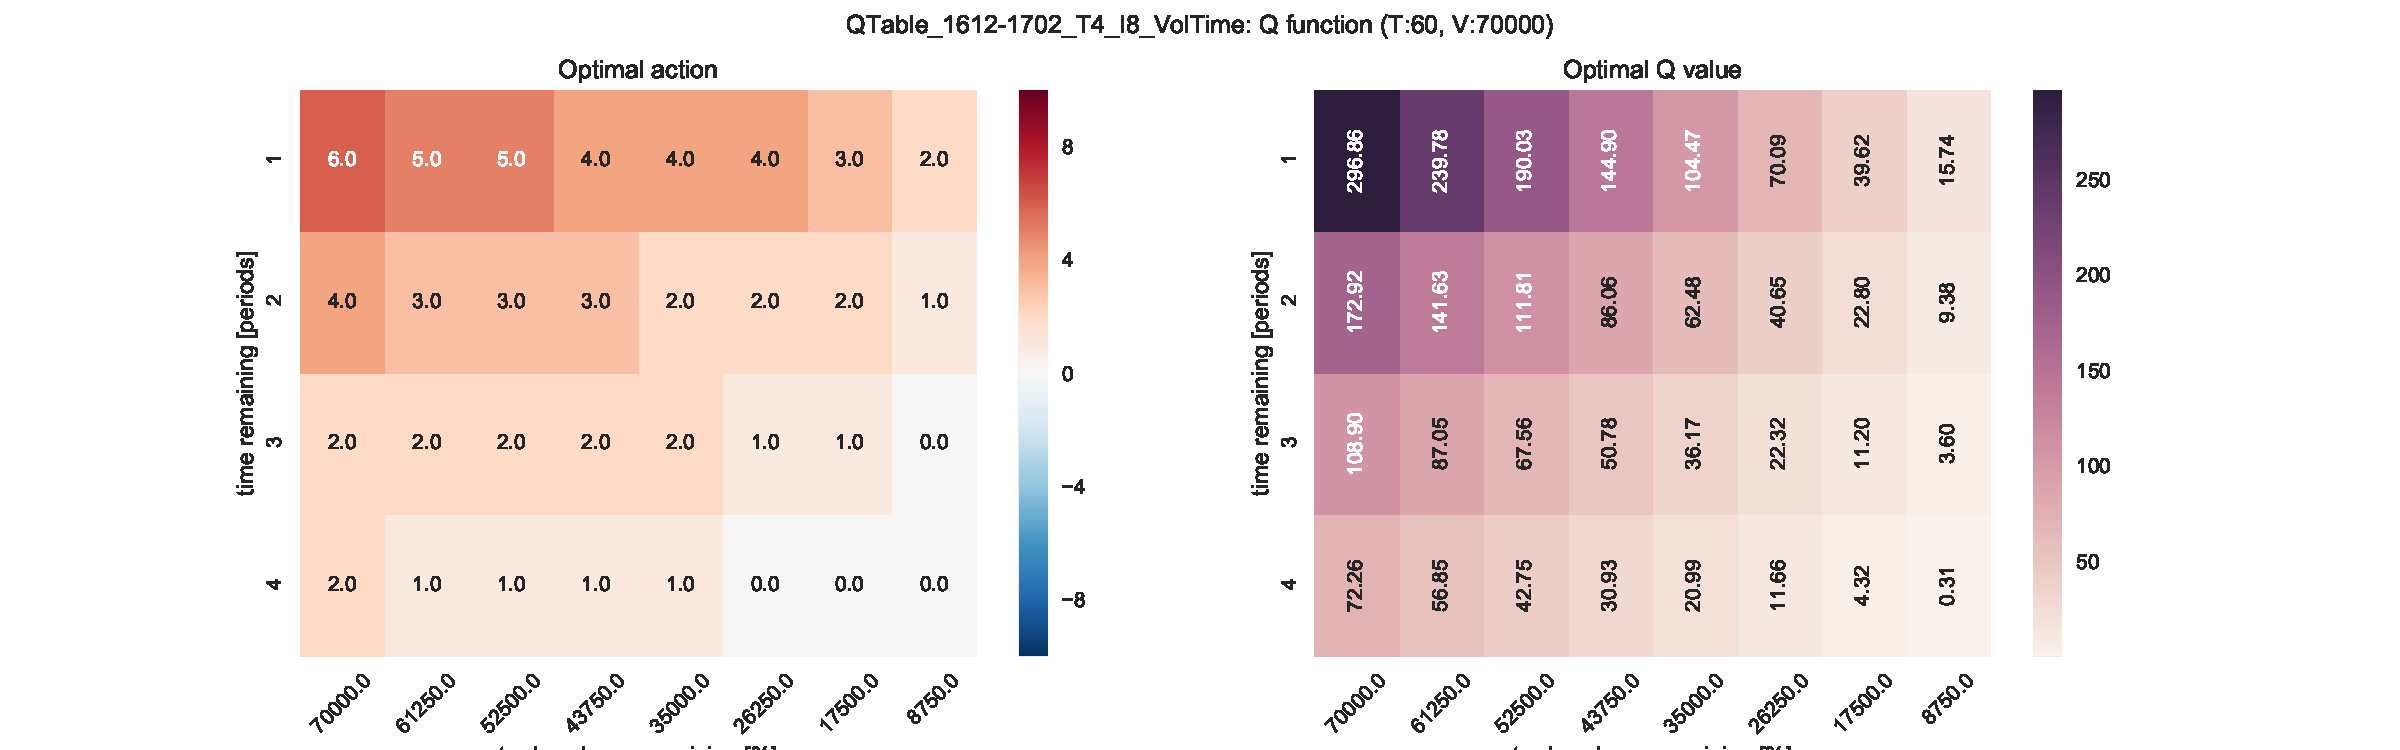
\includegraphics[width=0.8\textwidth]{content/drawings/heatmap_3months}
	\caption{Final State-Action function.}
	$T=4$ (60min), $I=8$ (70.000\$), L=15 ([-4, -3, \ldots{}, 9, 10])
	\label{fig:heatmap}
\end{figure}

\Cref{fig:heatmap} illustrates clearly, how the optimal strategy becomes more aggressive as time ceases and a large portion of the trading volume remains unexecuted.\\

\subsection{Incorporating preceding trades}
\label{chap:backwardapproach:precedingTrades}
In order to strengthen the Markov Property, \ie the assumption that states capture all relevant information from the history, the preceding trade history  (\ie the self-induced market impact) must be taken into account. \Cref{fig:differingmasterbooks} shows differing masterbook shapes, that can build the base of a simulated \lstinline!trading_period!, \eg if starting at $t=45min$ and a remaining trade volume of 17.500\$. \ref{fig:differingmasterbooks:NoSim} shows the original orderbook, as if no orders had been matched by our strategy. This version of the masterbook is queried by the original backward algorithm, potentially resulting in more passive trading aggressions, as it does not account for the self-induced impact on the market at all. \ref{fig:differingmasterbooks:SimMarketOrder} and \ref{fig:differingmasterbooks:SimEq} show two ideas, how the market impact can be incorporated. Both lead to different masterbook shapes and as such to different subsets of attainable prices.\\

\begin{figure}[ht]
	\centering
	\begin{subfigure}[t]{0.3\textwidth}
        		\centering
        		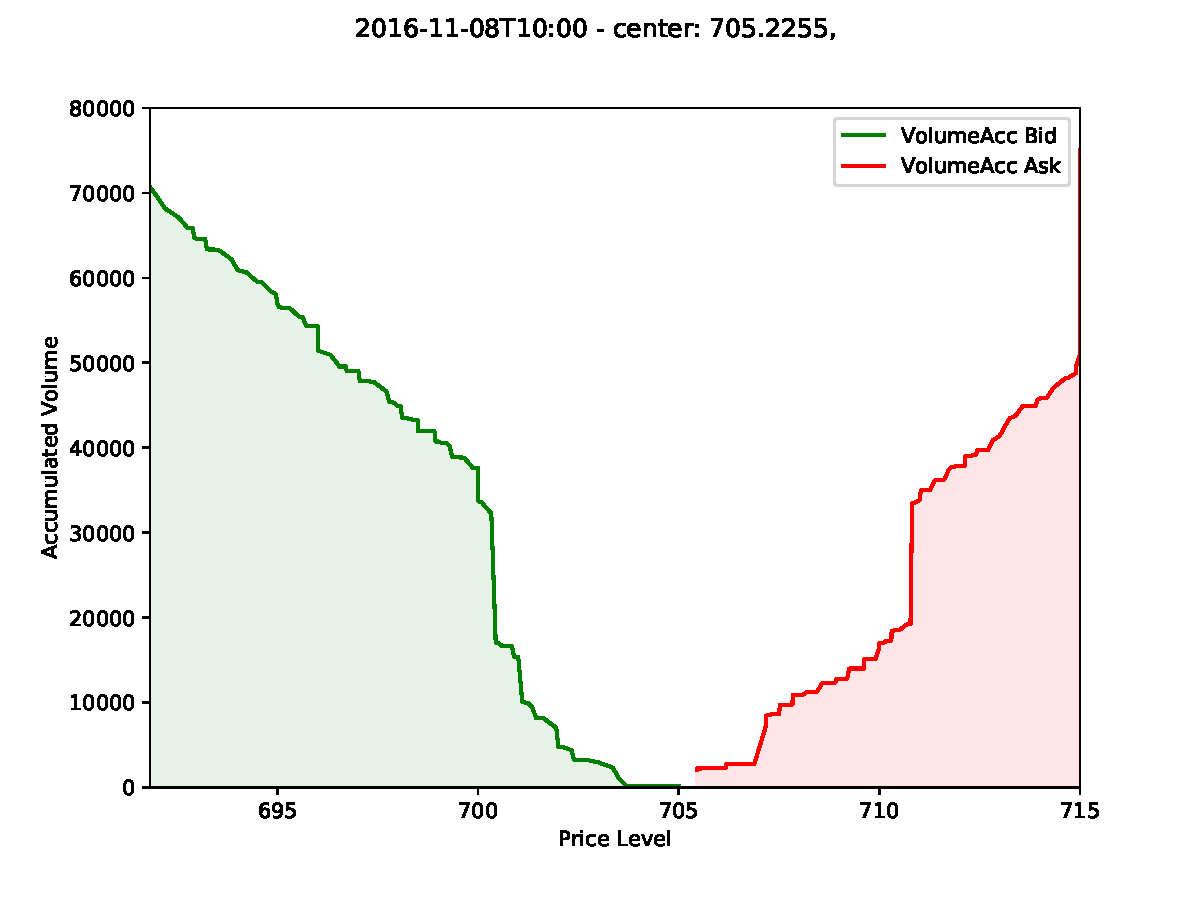
\includegraphics[width=\textwidth]{content/drawings/masterbook_customstart_NoSim}
        		\caption{Original Orderbook.}
		\label{fig:differingmasterbooks:NoSim}
    	\end{subfigure}
	\begin{subfigure}[t]{0.3\textwidth}
        		\centering
        		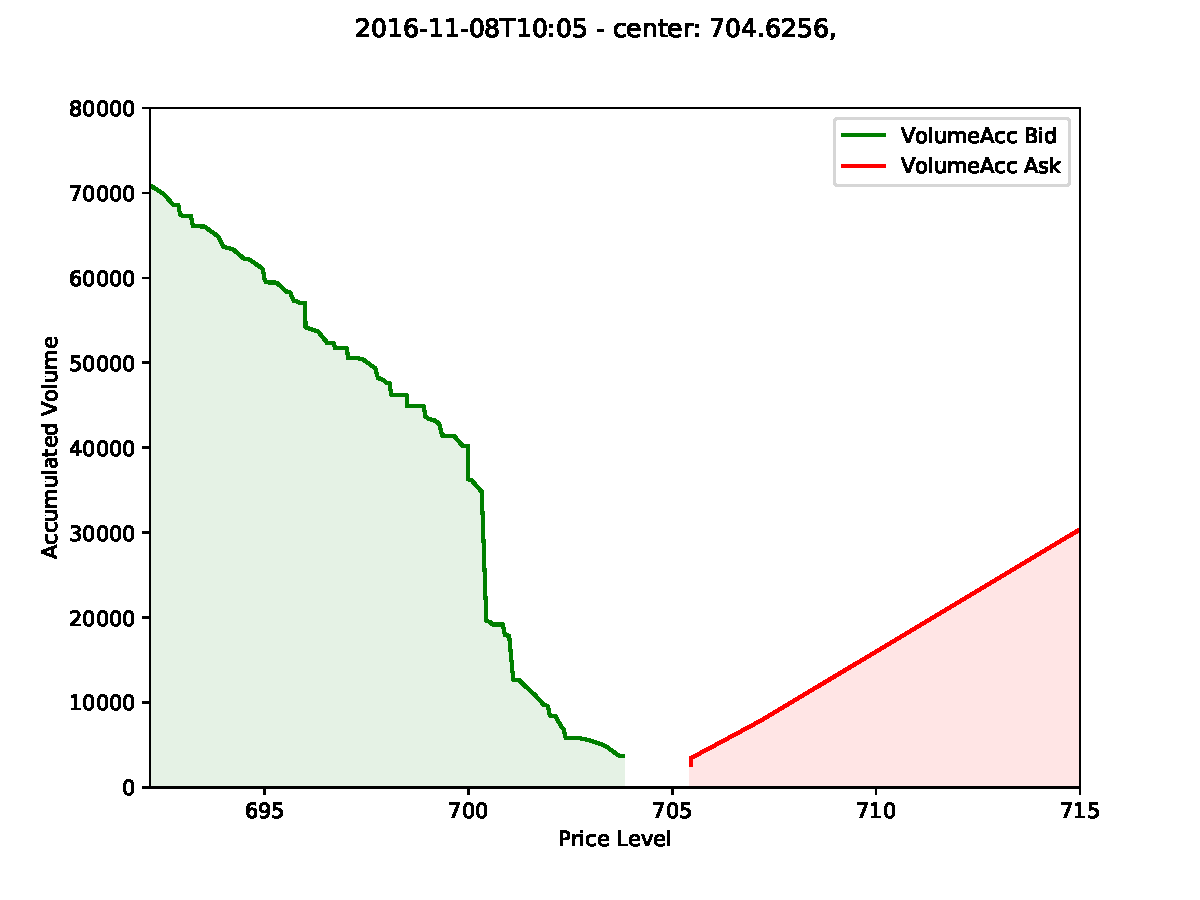
\includegraphics[width=\textwidth]{content/drawings/masterbook_customstart_SimMarketOrder}
        		\caption{Assuming 52.500 shares being matched at \lstinline!t=0!, then no further matches.}
		\label{fig:differingmasterbooks:SimMarketOrder}
    	\end{subfigure}%
	\begin{subfigure}[t]{0.3\textwidth}
        		\centering
        		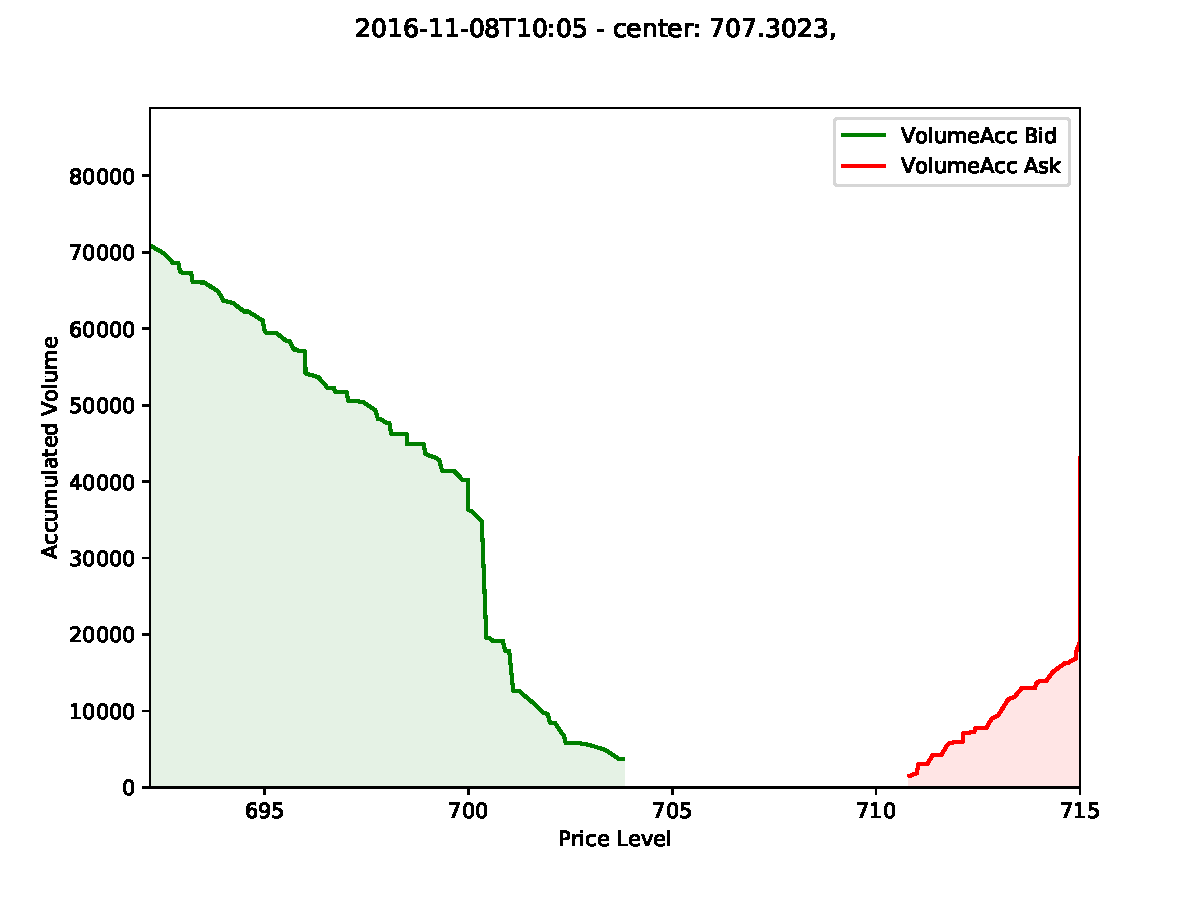
\includegraphics[width=\textwidth]{content/drawings/masterbook_customstart_SimEqual}
        		\caption{Assuming 52.500 shares being matched evenly at 1.166 shares per minute.}
		\label{fig:differingmasterbooks:SimEq}
    	\end{subfigure}%

	\caption{Different shaped masterbooks at \lstinline!t=45!.}
	The shapes differ, depending on the preceding trade history.
	\label{fig:differingmasterbooks}
\end{figure}

\Cref{alg:bruteforceimproved:pseudocode} shows a modified version of the original backward-learning algorithm. Prior to the actual trade simulations, the supposedly consumed trading volume is removed from the masterbook. The orders affected, are matched and removed from the masterbook evenly along the elapsed time, as indicated in \Cref{fig:differingmasterbooks:SimEq}.\\

\begin{algorithm}[H] 
 \caption{Optimal\_strategy, improved.}
     \SetAlgoLined
     \footnotesize
     
     \KwIn{V=70.000\$, H=60min, T=4, I=[12.5\%..100\%], L=[-4..10]}

\For{t=1 to T}{
    \While{not end of data}{
        Transform (orderbook) $\rightarrow o_1..o_R$\;
        \For{i=0 to I}{
            \For{a=0 to L}{
                 {\color{red}Incorporate preceding trade history}\;
                 Set $x = [t, i, o_1, ..., o_R]$\;
                    Simulate transition $x \rightarrow y$\;
                    Calculate immediate $\text{cost}_{im}(x, a)$\;
                    Look up argmax $\text{cost}(y, p)$\;
                    Update $\text{cost}([t, v, o_1, ..., o_R], a)$\;

            }
        }
        Select the highest-payout action argmax $\text{cost}(y, p)$ in every state $y$ to output optimal policy
    }
}
\label{alg:bruteforceimproved:pseudocode}
\end{algorithm}





\subsection{Separation of Sampling \& Learning Phases}
The process of sampling from training data and learning optimal state-action values is split into two independent phases, mostly due to performance\footnote{The backward sampling phase for the example mentioned in \Cref{chap:backwardlearning}, took roughly 10 hours, even though the work load was distributed among 24 CPU's.} reasons. In the \emph{sampling phase}, all possible combinations of actions and private variables are evaluated and stored as 5-tuples $sample=(state, action, cost, timestamp, new\_state)$. As market variables are supposedly not influenced by the agents behavior (see \Cref{chap:statespace}), it suffices to remember the orderbooks time point, to allow adjacent substitution of market variables.\\

Samples are stored as DataFrame and may be exported and reused by other agents\footnote{Agents should refer to the same environment settings, as samples collected from different environments (\eg trading horizon of $H=8min$ vs. $H=60min$) may not be compatible.}, as wished. This allows to skip the time consuming process of backward sampling. Before the action learning phase starts, the collected samples may be enhanced by a variety of market variables, discretized or untouched. The helper function \lstinline!addMarketFeatures_toSamples()! retrospectively adds market variables to the agents samples DataFrame.\\

If desired, features are discretized according to their individual value range.\\
\Eg a chosen resolution of 3, evenly transforms feature $o_m$ into $o_{m\_disc3}$, according to automatically determined boundaries: \\
0 (if $o_m< 1/3$ quantile), 1 (if $1/3 \leq o_m < 2/3$ quantile) and 2 (if $o_m \geq 2/3$ quantile). Boundaries arise from the training data and are applied to test data unaltered.\\

The learning phase starts hereinafter, whereas two types of \emph{orderbook agents} have been implemented and experimented with, each of which employ different techniques:

\begin{description}
\item[QTable\_Agent] : Dynamic Programming as described in \Cref{chap:backwardlearning}.\\
Expected state-values are stored in a simple lookup table, hence discretization of the state space is required. For each state, a vector of length $L=num\_actions$ is maintained, of which the first argmin refers to the optimal action. The \emph{QTable} does not generalize to previously unobserved states and returns the very first action (here -4) by default. For proper cost-updates an additional \emph{NTable} is maintained, referencing the particular number of observations made.\\
QTable and NTable entries are computed in an iterative manner. In the first round, all samples with \lstinline!time_left=1! are evaluated, in the second round all samples with \lstinline!time_left=2!, \etc The private variable \lstinline!volume! is discretized according to the specified resolution and linear cost scaling (see \Cref{chap:costs}) is performed.

\item[BatchTree\_Agent]: Tree-Based Batch Mode Reinforcement Learning \Cite{Ernst:2005:TreeBasedBatchModeRL}.\\
An ensemble of 400 decision trees, with a maximum allowed depth of 15 is fed with the full batch of samples simultaneously, no discretization required. $T$ Fitted-Q-learning rounds (see \Cref{chap:background:treebasedBatchRL}, \Cref{alg:fittedQiteration}) are performed, to completely allow expected costs to unfold over the given time horizon.\\
The state space is enlarged by an extra dimension for the chosen action. Predicting the optimal action to choose for a given state, the ensemble must predict $L=num\_actions$ q-values, from which the argmin refers to the optimal action.
\end{description}\bigskip

Each \emph{orderbook agents} inherits some commonly shared functionality from the super class \lstinline!class RL_Agent_Base!. This base class provides a consistent framework, allowing to swap the logic behind \lstinline!learn_from_samples! and \lstinline!predict! only, while general functionality like \lstinline!load!, \lstinline!save!, \lstinline!plot_heatmap_Q! and \lstinline!collect_samples! may be reused.\\

An \emph{orderbook agent} holds the environment parameters, used to initialize the \ac{OTS}. As such, different definitions for the optimal trading problem require different orderbook agents.






\section{Forward Learning}
\label{chap:forwardlearning}
In order to collect more realistic transition samples, an alternative, \emph{forward sampling} method is presented.

\subsection{Forward Sampling \& Learning}
Rather than examining all available actions on the great variety of combinational possibilities the state space has to offer, the forward approach repeatedly simulates trades in their entirety. The once again utilized \ac{OTS} always starts with $V=100\%$, but may be initialized at random start points (\eg \lstinline!t=0, t=15, t=30, t=45!) and keeps going until the full trade is executed.\\

As such, the obtained transitions stem from a more natural and furthermore fully continuous environment. Only actually attainable states, that could arise in the (simulated) reality, are used as transition start points, potentially increasing their significance. As major disadvantage, this forward sampling approach does not assure exhaustive exploration of the state space. A thorough exploration is not self-evident and must be supervised.\\

The pseudo-code of the forward sampling approach is shown in \Cref{alg:forward:pseudocode}. The algorithm iterates over the training data, starts $E$ exploration phases per orderbook window and follows an $\epsilon$-greedy exploration strategy. Each exploration phase starts with $\epsilon=1.0$ which finally decays to $\epsilon=0.05$ according to $\epsilon=0.05^{e/E}$.\\

\begin{algorithm}[H] 
 \caption{Forward sampling and learning approach.}
     \SetAlgoLined
     \footnotesize
     
     \KwIn{data, V=$70.000\$$, H=60min, T=4, L=[-4..10], E=60, retrain=256}

Shuffle(data)\;
Split data into chunks of length $retrain$

\While{not end of chunks}{
\For{orderbook window in chunks}{
Init OTS(orderbook\_window, V, H, T, L)\;
    \For{epoch=0 to E}{
        Reset OTS to $V=100\%$ and random time point (in H)\;
        \Repeat{$V=0\%$}{
        Set $x_t=[\text{time\_left}, \text{volume\_left}, o_1, ..., o_R]$\;
        Enquire $\epsilon$-greedy action from model\;
        \If{action chain led to an end state previously}{choose other action}
        Apply action\;
        Remember transition \{$x_t, action, cost, x_{t+1}$\}
        }
    }
    Retrain model from collected transitions (growing batch)
    }
}

\label{alg:forward:pseudocode}
\end{algorithm}\bigskip

If $\epsilon$-greedy proposes an actions, that previously led to an end state (\ie trade completed), an alternative action is sampled according to a gaussian distribution with its peak at the originally proposed action. Before the actual random draw, probabilities of all dead-end-actions are set to zero, to forestall pointless resampling. In case of repeatedly running into dead-ends (\eg \lstinline!max_dead_ends=4!) the exploration phase is aborted and continues with the next orderbook.\\

After every \lstinline!retrain! exploration phases, the new samples are fit into the agents model (\eg \lstinline!retrain=256!) and the updated model is used for future $\epsilon$-greedy exploration. Prior to the sampling phase, the training set is shuffled.\\

In contrast to the backward sampling method, market variables may be queried on the go, such that they entail the strategies impact. Because sample trajectories stem from a continuous state space function approximations prove handy. In this work, a RandomForestRegressor (\ie \ac{BT}) is utilized and retrained from scratch every \lstinline!retrain! exploration phases. The alternative approach of exploiting Neural Fitted Q-iteration \Cite{Riedmiller:2005:NFQ}, has been postphoned to future experiments.\\











\cleardoublepage{}